\subsection{Umsetzung des UI} 
Die grafische Darstellung der ermittelten Messdaten wird im folgenden Kapitel beschrieben.

\subsubsection{Abkapselung des Datenzugriffs}
Das Projekt wurde so aufgebaut, dass die Messdaten von einer grafischen Darstellung unabhängig sind.
Durch diese Unabhängigkeit konnte der ganze Prozess des Messens und Speicherns für sich implementiert werden.\\
\\
Als Abkapselung des grafischen User Interface wurde eine REST Schnittstelle entworfen, welche im Kapitel \ref{sec:rest} genauer beschrieben ist.
Mit dieser Schnittstelle wurde eine Möglichkeit geschaffen, die Messdaten zu lesen ohne direkt im Programm implementiert zu sein.\\
\\
Die Daten müssen allerdings vom Verwender aufbereitet werden.
Berechnungen wie zum Beispiel der täglichen Abweichung und der Abweichung seit Messbeginn müssen aus den lesbaren Daten berechnet werden.
Als lesbare Daten gelten folgende Punkte:
\begin{itemize}
    \item Name der Uhr
    \item Zeitstempel der Messung
    \item Absolute Zeit
    \item Referenzzeit während der Messung
    \item Temperatur und Feuchtigkeit
\end{itemize}
Die lesbaren Daten können direkt über die REST Schnittstelle abgefragt werden.
Lässt man dabei die Daten in ihrer rohen Form, erhält man einen JSON-Aufbau wie er in Kapitel \ref{sec:rest_struct} definiert ist.

\clearpage
\subsubsection{Mögliche Lösungsvariante}
Als Teil dieser Arbeit wurde ein möglicher Entwurf einer grafischen Benutzeroberfläche erarbeitet.\\
\\
Für die grafischen Elemente wird ein Bootstrap Template von Aigars Silkalns\footnote{Bootstrap Template von \cite{bootstrap}} verwendet.
Dieses Template steht unter der MIT Lizenz und kann daher frei verwendet werden.
Es bietet Snippets, Widgets und Custom Pages.\\
\\
Der Inhalt der Oberfläche wäre wie folgt definiert:
\begin{itemize}
    \item Oberer Teil \begin{itemize}
        \item Anzeige von Temperatur
        \item Anzeige von Feuchtigkeit
        \item Abweichung pro Tag
        \item Abweichung seit Messbeginn
    \end{itemize}
    \item Linker Teil
    \begin{itemize}
        \item Verlauf der Abweichung über das Jahr
    \end{itemize}
    \item Rechter Teil
    \begin{itemize}
        \item Liste mit den Messdaten eines Tages
    \end{itemize}
\end{itemize}
Als zusätzliches Feature kann zum Beispiel eine Filterung nach Datum oder Uhr erfolgen.
Dabei würden alle Anzeigen, ausser der ''Abweichung seit Messbeginn'', aktualisiert.
Der Standardfilter wäre der letzte gemessene Tag.\\
\\
Ein solcher Lösungsvorschlag könnte wie in Bild \ref{fig:ui_draft} aussehen.

\begin{figure}[H]
    \centering
    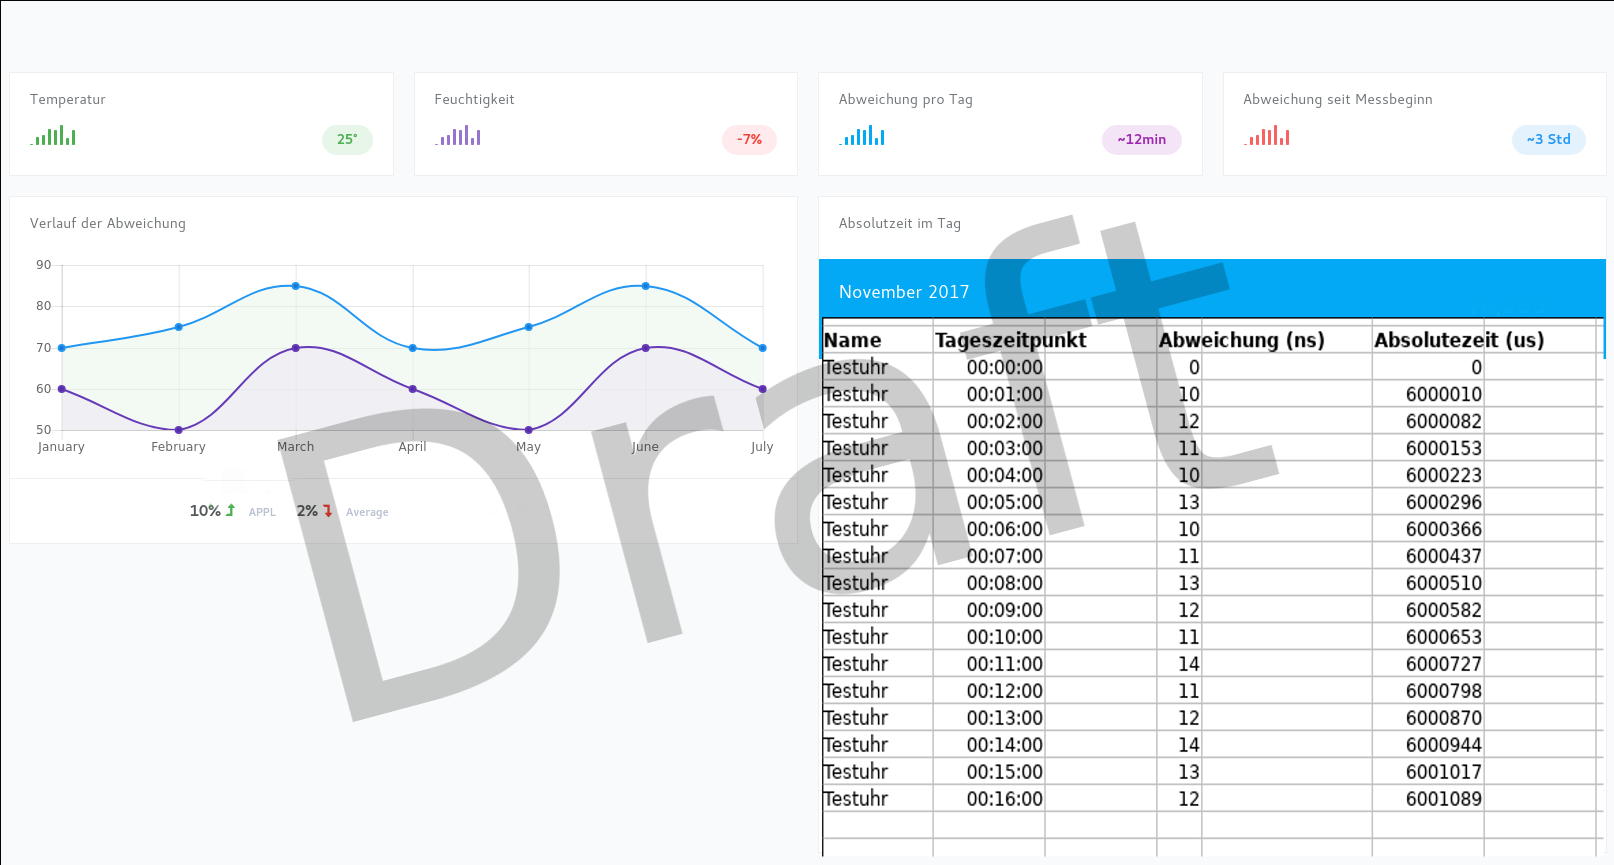
\includegraphics[width=\textwidth]{webclient_draft}
    \caption{Entwurf einer grafischen Oberfläche}
    \label{fig:ui_draft}
\end{figure}